\chapter{Conclusão}
    \label{chp:Conclusão}

    %Justificativa -> tema
    Este trabalho de pesquisa foi iniciado diante da necessidade de se investigar se seria possível dar mais liberdade no desenvolvimento de aplicações para um robô industrial com controladora aberta, atendendo inclusive a demanda do Laboratório de Robótica do CEFET-MG.
    
    %Objetivo Geral (se foi atendido)
    Diante disso, o objetivo geral do trabalho foi desenvolver um software com um arranjo cliente servidor que estenda a liberdade que a solução da fabricante proporciona aos programadores de robôs industriais. Tal software foi desenvolvido e o objetivo geral foi atingido.
    
    %Cada um dos objetivos Específicos (se foi atingido)
    O protocolo de comunicação TCP/IP para enviar e receber variáveis referentes aos ângulos de juntas do robô foi criado, permitindo que softwares clientes programados nas mais diversas linguagens de programação e sistemas operacionais se comuniquem fazendo uso dele, atingindo assim o primeiro objetivo específico.
    
    A função que comunica com a controladora do robô, salvando e enviando informações da memória, foi implementada, bem como a função que se comunica com o software cliente, salvando e enviando informações da memória, atingindo assim o segundo e o terceiro objetivos específicos.

    E por fim, o problema gerado pelo assincronismo da comunicação do OpenServer com a controladora e o programa cliente foi solucionado através do uso de ponteiros inteligentes para salvar as informações na memória, garantindo assim que não ocorra problemas na atribuição de valores na memória no momento da leitura dos mesmos. Assim, o último objetivo específico foi atingido.
        
    %Relato das descobertas dos objetivos específicos
    %Foi descoberto que 
    
    %Hipótese (Qual foi? Confirmada ou refutada)
    Partiu-se da hipótese que é possível desenvolver um software que se comunique ao mesmo tempo com a controladora do robô e com um programa cliente, porém em taxas diferentes, sendo este dispositivo de outra arquitetura e o software programado em uma linguagem diferente e rodando em um sistema operacional diferente. A hipótese foi confirmada e tal software desenvolvido.
    
    %Limitações: Dificuldades encontradas - Limitações da pesquisa
    Uma limitação atual da pesquisa está sendo diagnosticar o gargalo do sistema que impede a comunicação de ocorrer a uma taxa menor que \SI{2}{\milli\second} de forma estável.
    
    %Recomendações: Consequência das dificuldades, recomendar continuidade
    Uma forma de superar esse gargalo seria desenvolver um programa cliente mais simples específico para coleta de dados de taxa de amostragem e implementar um protocolo adicional de comunicação que envie informações direto da memória RAM sem os converter em \textit{strings}, como foi feito nesse trabalho
    
    \section{Perspectivas futuras}
        
        Com objetivo de atingir taxas de comunicação maiores, está em fase de estudos o desenvolvimento de protocolos de comunicação mais otimizados com base em \ac{TCPIP}. Por exemplo, criando uma nova modalidade, desta vez de forma síncrona, que envie dados ao mesmo tempo que recebe, ao invés de usar a forma assíncrona, que aguarda o recebimento de um dado para enviar o próximo. Espera-se que isso dobre a taxa de comunicação.
        
        Outra modalidade em fase de estudos seria, como já citado, transmitir os dados binários direto da memória RAM. Essa modalidade talvez seja menos compatível com outras linguagens de programação, mas é focada em aplicações com a necessidade específica de taxas de amostragens mais altas. 
        
        Está sendo elaborado o desenvolvimento um programa cliente do OpenSever que adiciona ao sistema robótico uma malha de controle baseada em visão computacional. Uma câmera afixada no efetuador do robô filma uma figura de referência, o software cliente processa a imagem e gera as referências que são enviados ao OpenServer, de forma a manter constante a pose (posição e orientação) do manipulador robótico em relação à pose da figura de referência. Dessa maneira, é adicionada uma câmera à estrutura desenvolvida, conforme é representado na Figura~\ref{pespectiva}, onde (1) representa a câmera e (2) a figura de referência.
    
        \begin{figure}[ht]
            \centering
            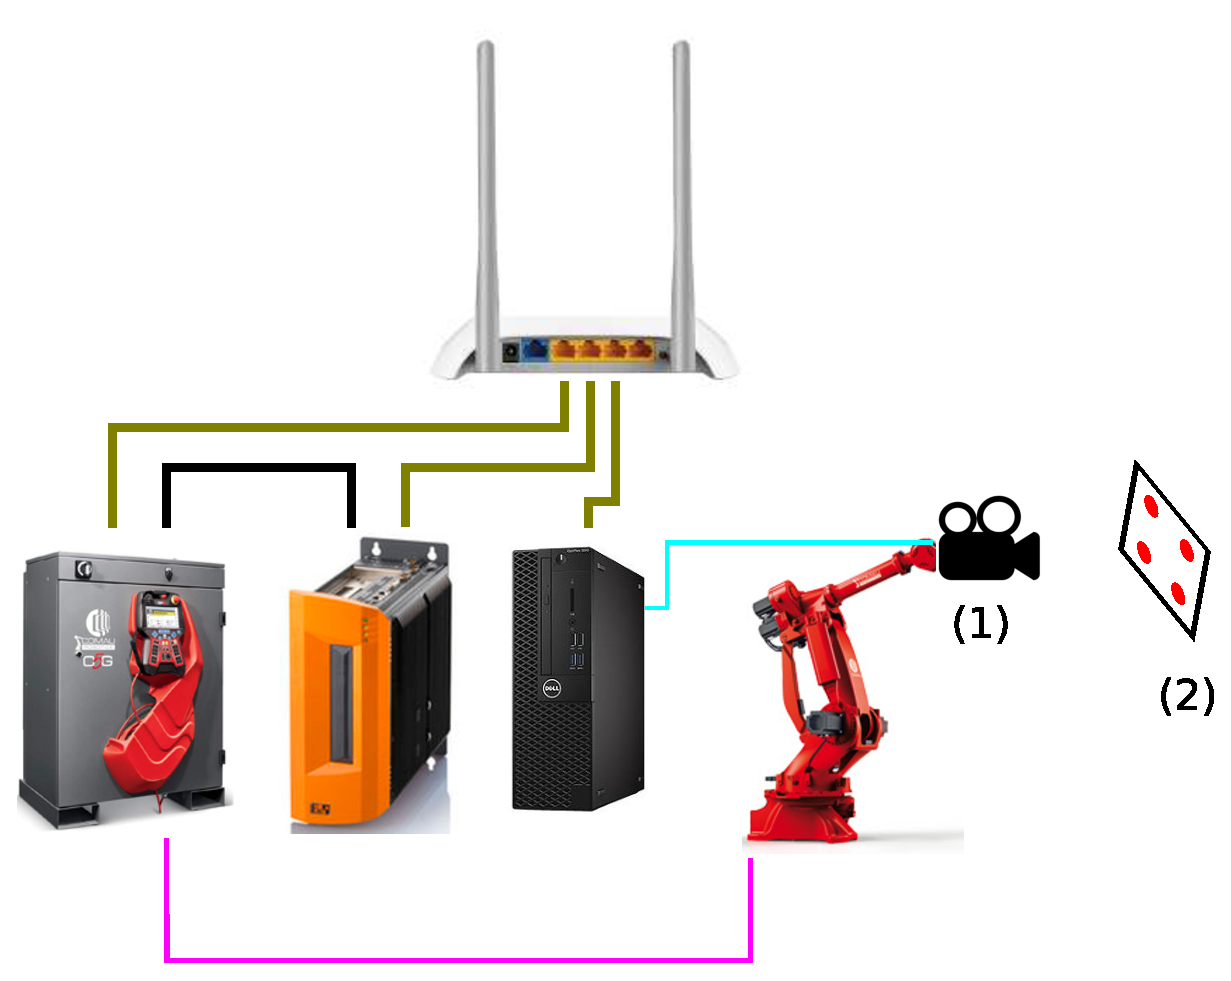
\includegraphics[width=\columnwidth]{imagens/pespectiva.eps}
            \small 
            \centering 
            \caption{Estrutura proposta para utilização do OpenServer}
            \label{pespectiva}
        \end{figure}        
